\documentclass{../talk}

\title{Testing Bell's inequality with entangled photons}
\author[Iago B. Mendes]{Iago B. Mendes \\ Lab partner: Anya Molodtsova}
\date{May 8, 2025}

\newcommand{\ket}[1]{| #1 \rangle}
\renewcommand{\deg}{^\circ}

\begin{document}

\maketitle

\section{Introduction}

\begin{frame}{Motivation}
  \begin{itemize}
    \item 1935: Einstein-Podolsky-Rosen (EPR) paradox
      \begin{itemize}
        \item Quantum mechanics (QM) is incomplete $\Rightarrow$ allows for ``spooky action at a distance''
        \item Local hidden variable theories (HVT) could explain entangled states
      \end{itemize}
    \item<2-> 1964: Bell's inequality
      \begin{itemize}
        \item Experimentally testable way to distinguish between QM and HVT
      \end{itemize}
    \item<3-> 1972: Freedman-Clauser experiment
      \begin{itemize}
        \item First experimental test of Bell's inequality
        \item Used entangled photons
      \end{itemize}
    % \item<4-> 2002: Dehlinger et al.'s experiment for undergraduate laboratory settings
    % \item<5-> 2004: Burton Betchart's Oberlin Honors Thesis
    % \item<6-> 2025: This experiment
  \end{itemize}
\end{frame}

\section{Theory}

\begin{frame}{Entangled photons}
  \begin{itemize}
    \item Created in a pair of beta barium borate (BBO) crystals,
    \item Nonlinear optic properties
      \begin{center}
        1 pump photon $\to$ 2 entangled photons
      \end{center}
  \end{itemize}
  \begin{figure}
    \centering
    \includegraphics[width=0.5\textwidth]{assets/photon-conversion.png}
    \caption{Reproduced from lab manual.}
  \end{figure}
\end{frame}

\begin{frame}{Entangled photons (continued)}
  \begin{itemize}
    \item Entangled state:
      \begin{equation}
        \ket{\psi} = \cos\theta_l \ket{HH} + e^{i\phi} \sin\theta_l \ket{VV}
      \end{equation}
    \item Maximum entanglement: $\theta_l = 45\deg$, $\phi = 0\deg$
      \begin{equation}
        \ket{\psi_\text{max}} = \frac{1}{\sqrt{2}} \left( \ket{HH} + \ket{VV} \right)
      \end{equation}
  \end{itemize}
\end{frame}

\begin{frame}{Detector polarizers}
  \begin{itemize}
    \item Photon detections at angles $\alpha$ and $\beta$
    \item Probability of both being ``vertical'':
      \begin{equation}
        P_{VV}(\alpha, \beta) = \sin^2\alpha \sin^2\beta \cos^2\theta_l + \cos^2\alpha \cos^2\beta \sin^2\theta_l + \frac{1}{4} \sin2\alpha \sin2\beta \sin2\theta_l \cos\phi_m
      \end{equation}
  \end{itemize}
  \begin{figure}
    \centering
    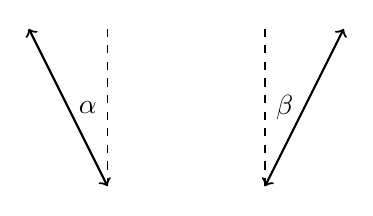
\begin{tikzpicture}
      \draw[dashed] (-1,-1) -- (-1,1);
      \draw[<->, thick] (-1,-1) -- (-2,1);
      \node at (-1.25,0) {$\alpha$};

      \draw[dashed] (1,-1) -- (1,1);
      \draw[<->, thick] (1,-1) -- (2,1);
      \node at (1.25,0) {$\beta$};
    \end{tikzpicture}
    \caption{}
  \end{figure}
\end{frame}

% \begin{frame}{Predictions for maximal entanglement}
%   \begin{itemize}
%     \item Quantum mechanics:
%       \begin{equation}
%         P^\text{QM}_{VV}(\alpha, \beta) = \frac{1}{2} \cos^2(\beta - \alpha)
%       \end{equation}
%     \item Local hidden variable theories (HVT):
%       \begin{equation}
%         P^\text{HVT}_{VV}(\alpha, \beta) = \frac{1}{2} - \frac{|\beta - \alpha|}{\pi}
%       \end{equation}
%   \end{itemize}
% \end{frame}

\begin{frame}{Bell's inequality}
  \begin{itemize}
    \item John Bell (1964) found an inequality that must be true for any HVT
      \begin{equation}\label{eq:Bell-inequality}
        S \leq 2
      \end{equation}
    \item Definitions:
      \begin{align}
        S &\equiv E(a,b) - E(a,b') + E(a',b) + E(a',b') \\
        E(\alpha,\beta) &\equiv P_{VV}(\alpha,\beta) + P_{VV}(\alpha_\perp,\beta_\perp) - P_{VV}(\alpha,\beta_\perp) - P_{VV}(\alpha_\perp,\beta)
      \end{align}
  \end{itemize}
  \begin{figure}
    \centering
    \includegraphics[width=0.225\textwidth]{assets/angles.png}
    \caption{$a = -45\deg$, $b = -22.5\deg$, $a = 0\deg$, and $b' = 22.5\deg$. Reproduced from lab manual.}
  \end{figure}
\end{frame}

\begin{frame}{Violation of Bell's inequality}
  \begin{itemize}
    \item In the {\bf maximally entangled state}, quantum mechanics predicts
      \begin{equation}
        S > 2
      \end{equation}
    \item Violation of Bell's inequality $\Rightarrow$ test of quantum mechanics
    \item Note: quantum mechanics still allows $S \leq 2$ for other states
  \end{itemize}
\end{frame}

\section{Methods}

\begin{frame}{Experimental setup}
  \begin{itemize}
    \item Half-wave plate: rotates polarization to set $\theta_l \approx 45\deg$
    \item Quarter-wave plate: corrects phase shift $\phi_m \approx 0$
  \end{itemize}
  \begin{figure}
    \centering
    \includegraphics[width=0.8\textwidth]{assets/setup.png}
    \caption{Reproduced from lab manual.}
  \end{figure}
\end{frame}

\section{Results}

\begin{frame}{Analysis of state}
  \begin{itemize}
    \item Model for number of coincidences:
      \begin{equation}
        N(\alpha,\beta) = A (\sin^2\alpha \sin^2\beta \cos^2\theta_l + \cos^2\alpha \cos^2\beta \sin^2\theta_l + \frac{1}{4} \sin2\alpha \sin2\beta \sin2\theta_l \cos\phi_m) + C
      \end{equation}
      4 parameters: $A$, $C$, $\theta_l$, $\phi_m$
    \item 2 approaches:
      \begin{enumerate}
        \item Strategic measurements $\Rightarrow$ find parameters analytically
        \item More measurements $\Rightarrow$ fit model
      \end{enumerate}
  \end{itemize}
\end{frame}

\begin{frame}{Analytic check}
  \begin{itemize}
    \item 5 measurements taken with $T = 60$ s (less accurate)
  \end{itemize}
  \begin{align}
    C &= N(0\deg, 90\deg) &&\Rightarrow C = 4(2) \\
    A &= N(0\deg, 0\deg) + N(90\deg, 90\deg) - 2 C &&\Rightarrow A = 19(6) \\
    \tan^2\theta_l &= \frac{N(90\deg,90\deg) - C}{N(0\deg,0\deg) - C} &&\Rightarrow \theta_l = 55(8)\deg \\
    \cos\phi_m &= \frac{1}{\sin 2\theta_l} \left( 4 \frac{N(45\deg, 45\deg) - C}{A} - 1 \right) &&\Rightarrow \cos\phi_m = 2(1) \\ \notag
  \end{align}
\end{frame}

\begin{frame}{Fit model}
  \begin{itemize}
    \item 16 measurements taken with $T = 8$ min (more accurate)
    \item Used {\tt SciPy}'s {\tt least\_squares} procedure to fit model to data
  \end{itemize}
  \begin{align}
    A &= 200(20) \\
    \theta_l &= 25(4)\deg \\
    \phi_m &= -0.003\deg \pm 300000\deg \\
    C &= 20(7)
  \end{align}
\end{frame}

\begin{frame}{State models}
  \begin{itemize}
    \item Corrected model: keep everything from fit model, but set $\theta_l = 45\deg$
  \end{itemize}
  \begin{figure}
    \centering
    \includegraphics[width=\textwidth]{analysis/state.pdf}
    \caption{}
  \end{figure}
\end{frame}

\begin{frame}{Bell's inequality}
  \begin{itemize}
    \item Using 16 measurements:
      \begin{equation}
        S = 1.8(1)
      \end{equation}
      $\Rightarrow$ not helpful (doesn't prove anything)
    \item<2-> Using corrected model:
      \begin{equation}
        S = 2.0(1)
      \end{equation}
      $\Rightarrow$ closer to the limit, but large uncertainty doesn't let us draw any conclusions
  \end{itemize}
\end{frame}

\section{Conclusion}

\begin{frame}{Summary}
  \begin{itemize}
    \item Used entangled photons to test Bell's inequality
    \item Not able to draw significant conclusions due to...
      \begin{enumerate}
        \item Photons not being in a maximally entangled state
        \item Large uncertainty in measurements
      \end{enumerate}
    \item<2-> Possible improvements:
      \begin{enumerate}
        \item Preparation of state
          \begin{itemize}
            \item Calibration and alignment of setup
            \item New BBO crystal (it was cracked)
          \end{itemize}
        \item Accuracy
          \begin{itemize}
            \item More coincidences
            \item Longer duration
          \end{itemize}
      \end{enumerate}
  \end{itemize}
\end{frame}

\begin{frame}{The end}
  \textbf{\Large Thank you! Any questions?}
  
  \hrulefill
\end{frame}

\end{document}
